\subsection{Additional Analysis of Hydrography Products}
\label{sec:appendix-hydrography-results}

Figures~\ref{fig:appendix-dt-window-hydrorivers} through~\ref{fig:appendix-dt-window-grit} repeat the histogram of Figure~\ref{fig:dt_window_histogram} for each hydrography product individually.
Every reach is given $k = Length / velocity$ with a constant flood wave celerity of 1~m/s and $x = 0.25$, the same assumptions as the combined histogram.
Each bar is the percentage of the product's reaches whose range of valid time steps from Equation~\ref{eq:validity-conditions} includes any $\Delta t$ in the bin.
All six figures share one vertical scale.

The time step valid for the most reaches follows the reach lengths summarized in Table~\ref{tab:hydrography-properties}.
It is between 21 and 33 minutes for HydroSHEDS~v2 and NHDPlus~V2, 42 to 53 minutes for HydroRIVERS and TDX-Hydro, and 1.8 to 2.8 hours for MERIT-Basins and GRIT.
No time step is valid for more than 54\% of the reaches of any product.
A time step suited to one product is poorly suited to another.
At a 5-minute time step, about 20\% of HydroSHEDS~v2 reaches and 18\% of NHDPlus~V2 reaches are valid compared to 3\% of MERIT-Basins reaches.
At a 2-hour time step, 52\% of MERIT-Basins reaches are valid compared to 6\% of HydroSHEDS~v2 reaches.

\begin{figure}[htbp]
    \centering
    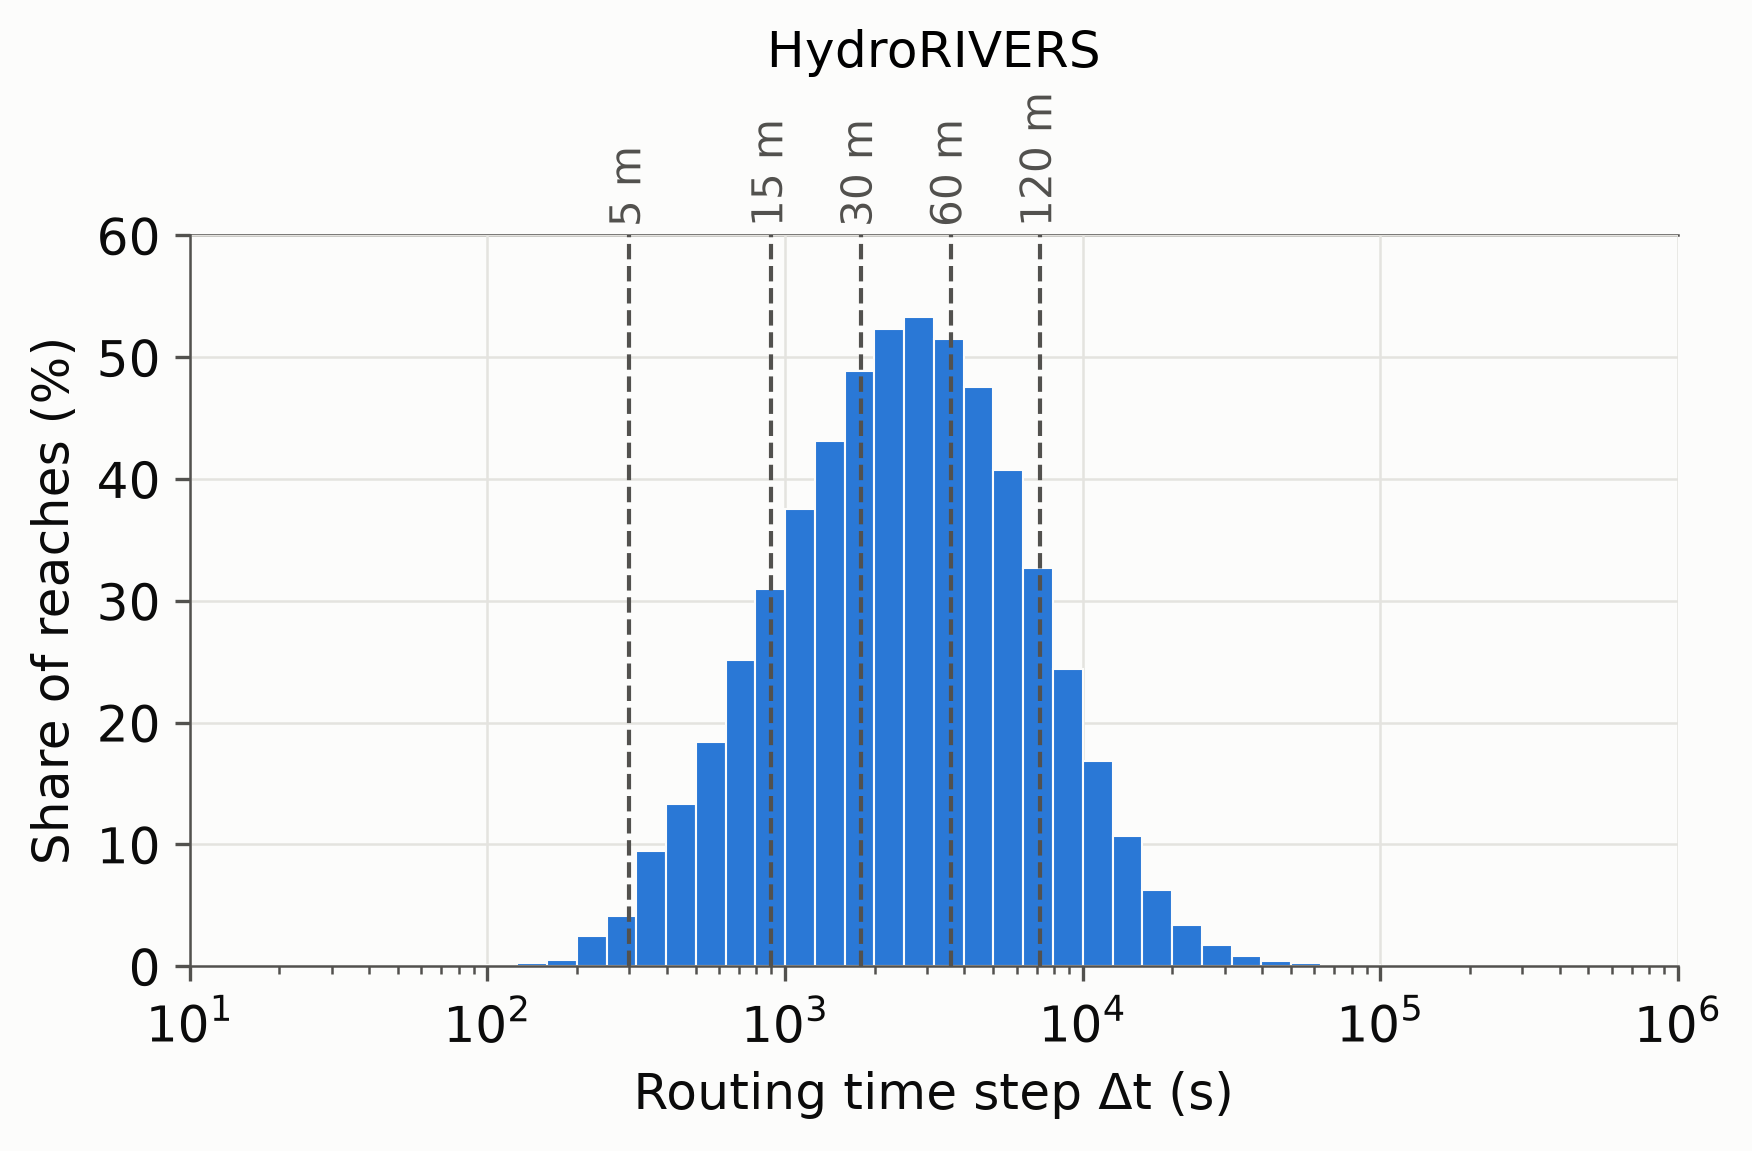
\includegraphics{../figures/dt_window_histogram_hydrorivers}
    \caption{Percentage of HydroRIVERS reaches with all positive Muskingum coefficients in each bin of routing time steps, assuming a constant flood wave celerity of 1~m/s and $x = 0.25$.}
    \label{fig:appendix-dt-window-hydrorivers}
\end{figure}

\begin{figure}[htbp]
    \centering
    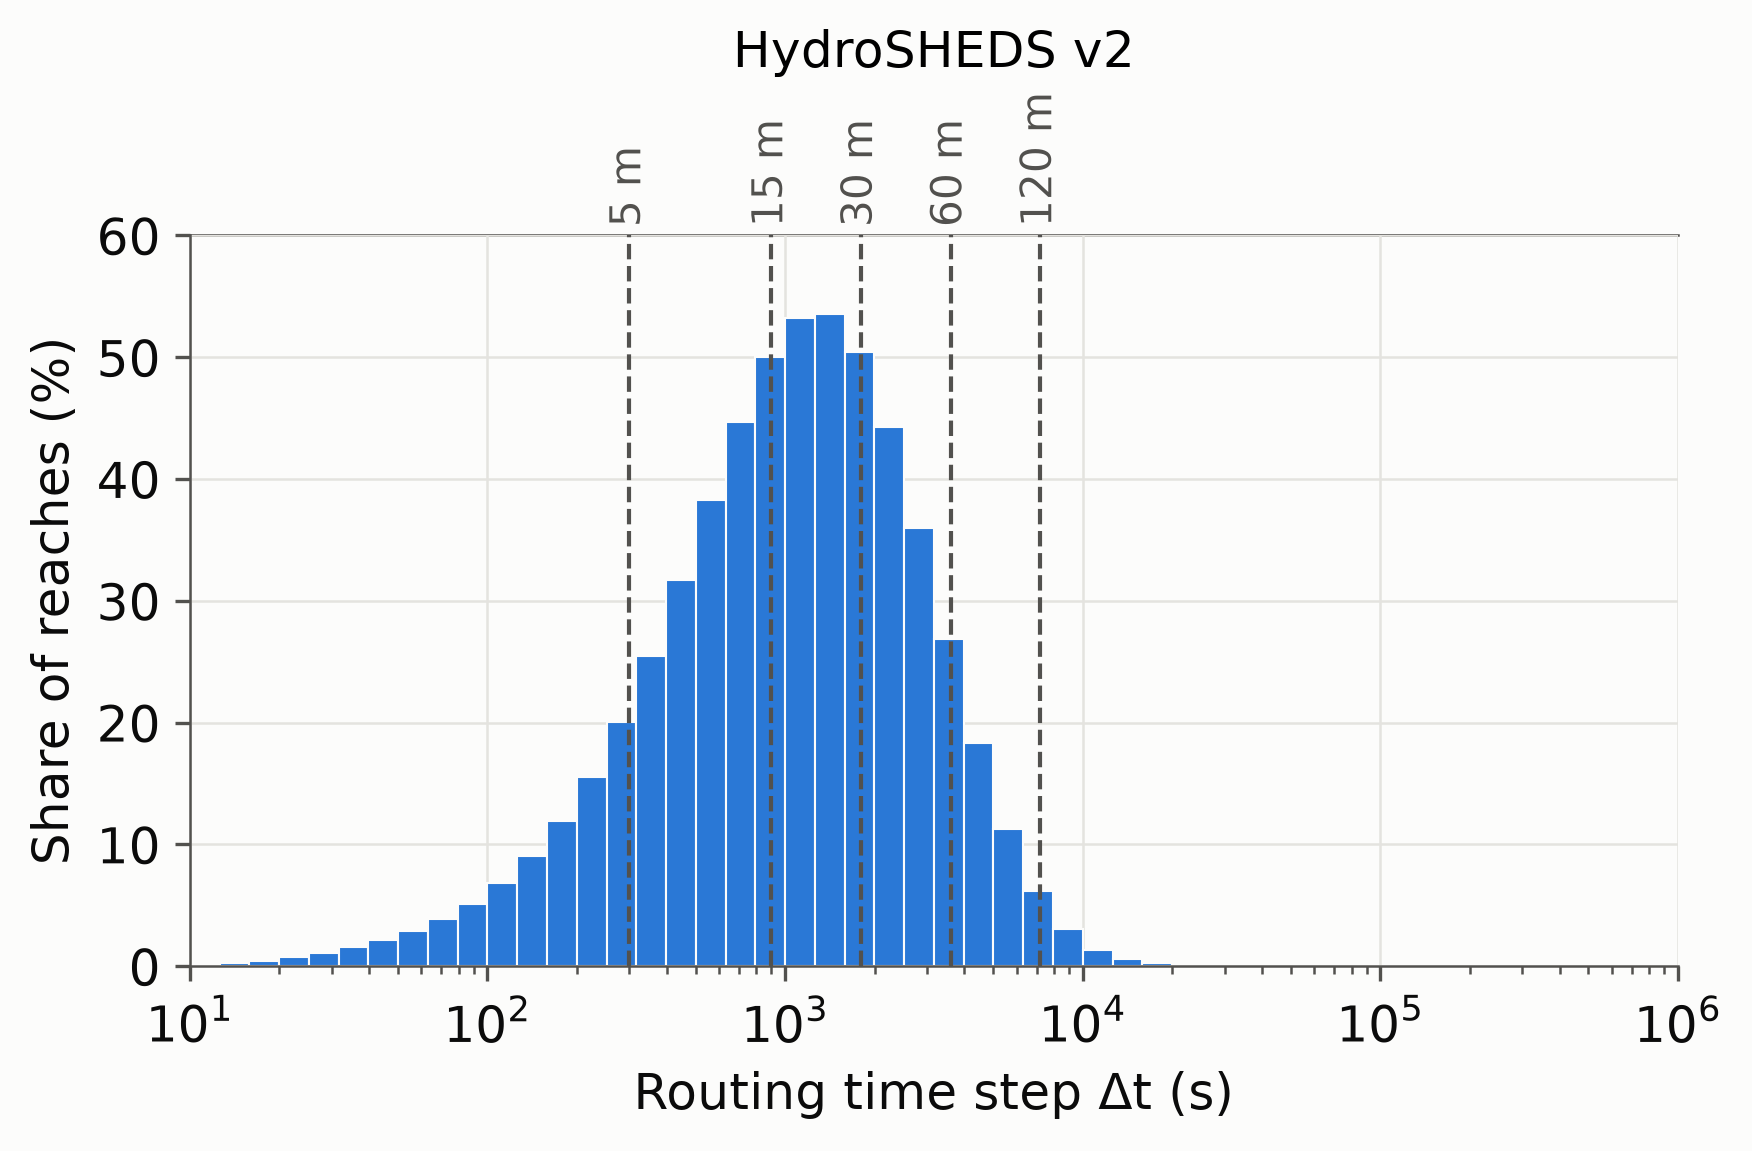
\includegraphics{../figures/dt_window_histogram_hydrosheds-v2}
    \caption{Percentage of HydroSHEDS~v2 reaches with all positive Muskingum coefficients in each bin of routing time steps, assuming a constant flood wave celerity of 1~m/s and $x = 0.25$.}
    \label{fig:appendix-dt-window-hydrosheds-v2}
\end{figure}

\begin{figure}[htbp]
    \centering
    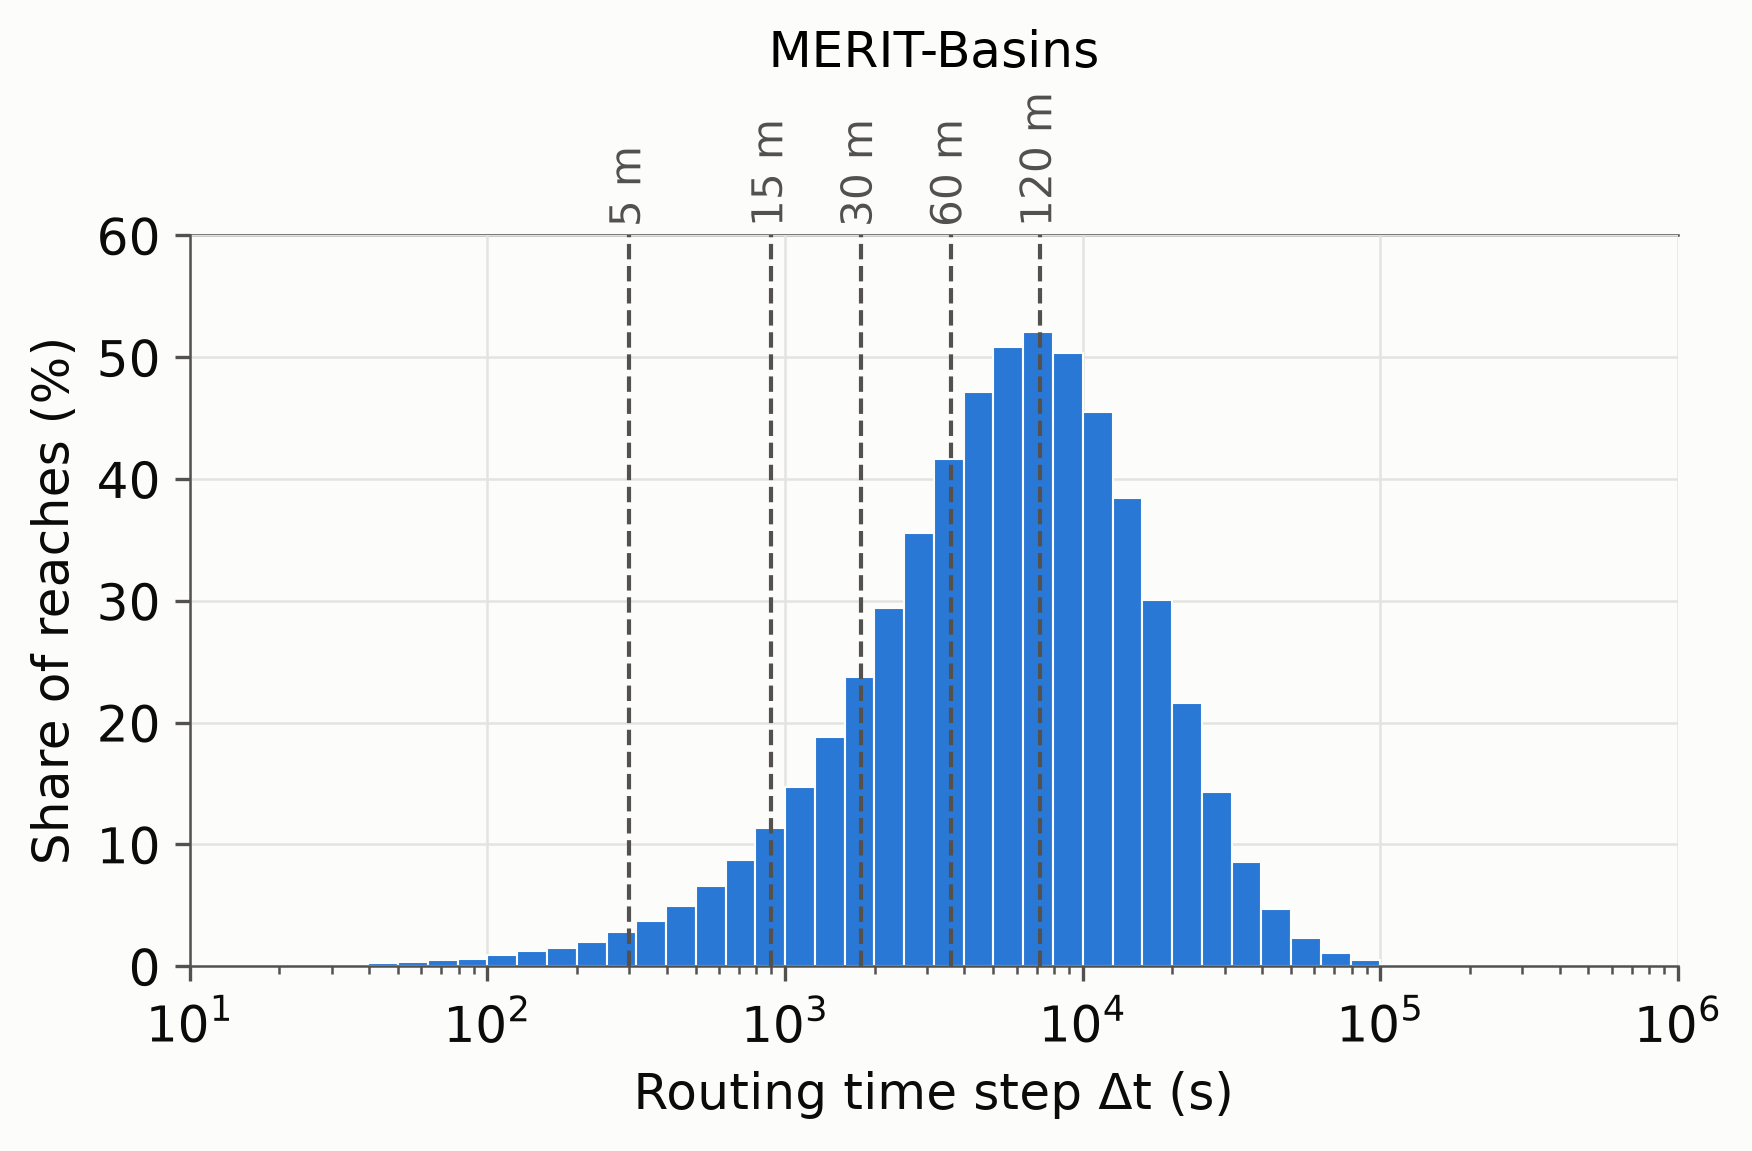
\includegraphics{../figures/dt_window_histogram_merit-basins}
    \caption{Percentage of MERIT-Basins reaches with all positive Muskingum coefficients in each bin of routing time steps, assuming a constant flood wave celerity of 1~m/s and $x = 0.25$.}
    \label{fig:appendix-dt-window-merit-basins}
\end{figure}

\begin{figure}[htbp]
    \centering
    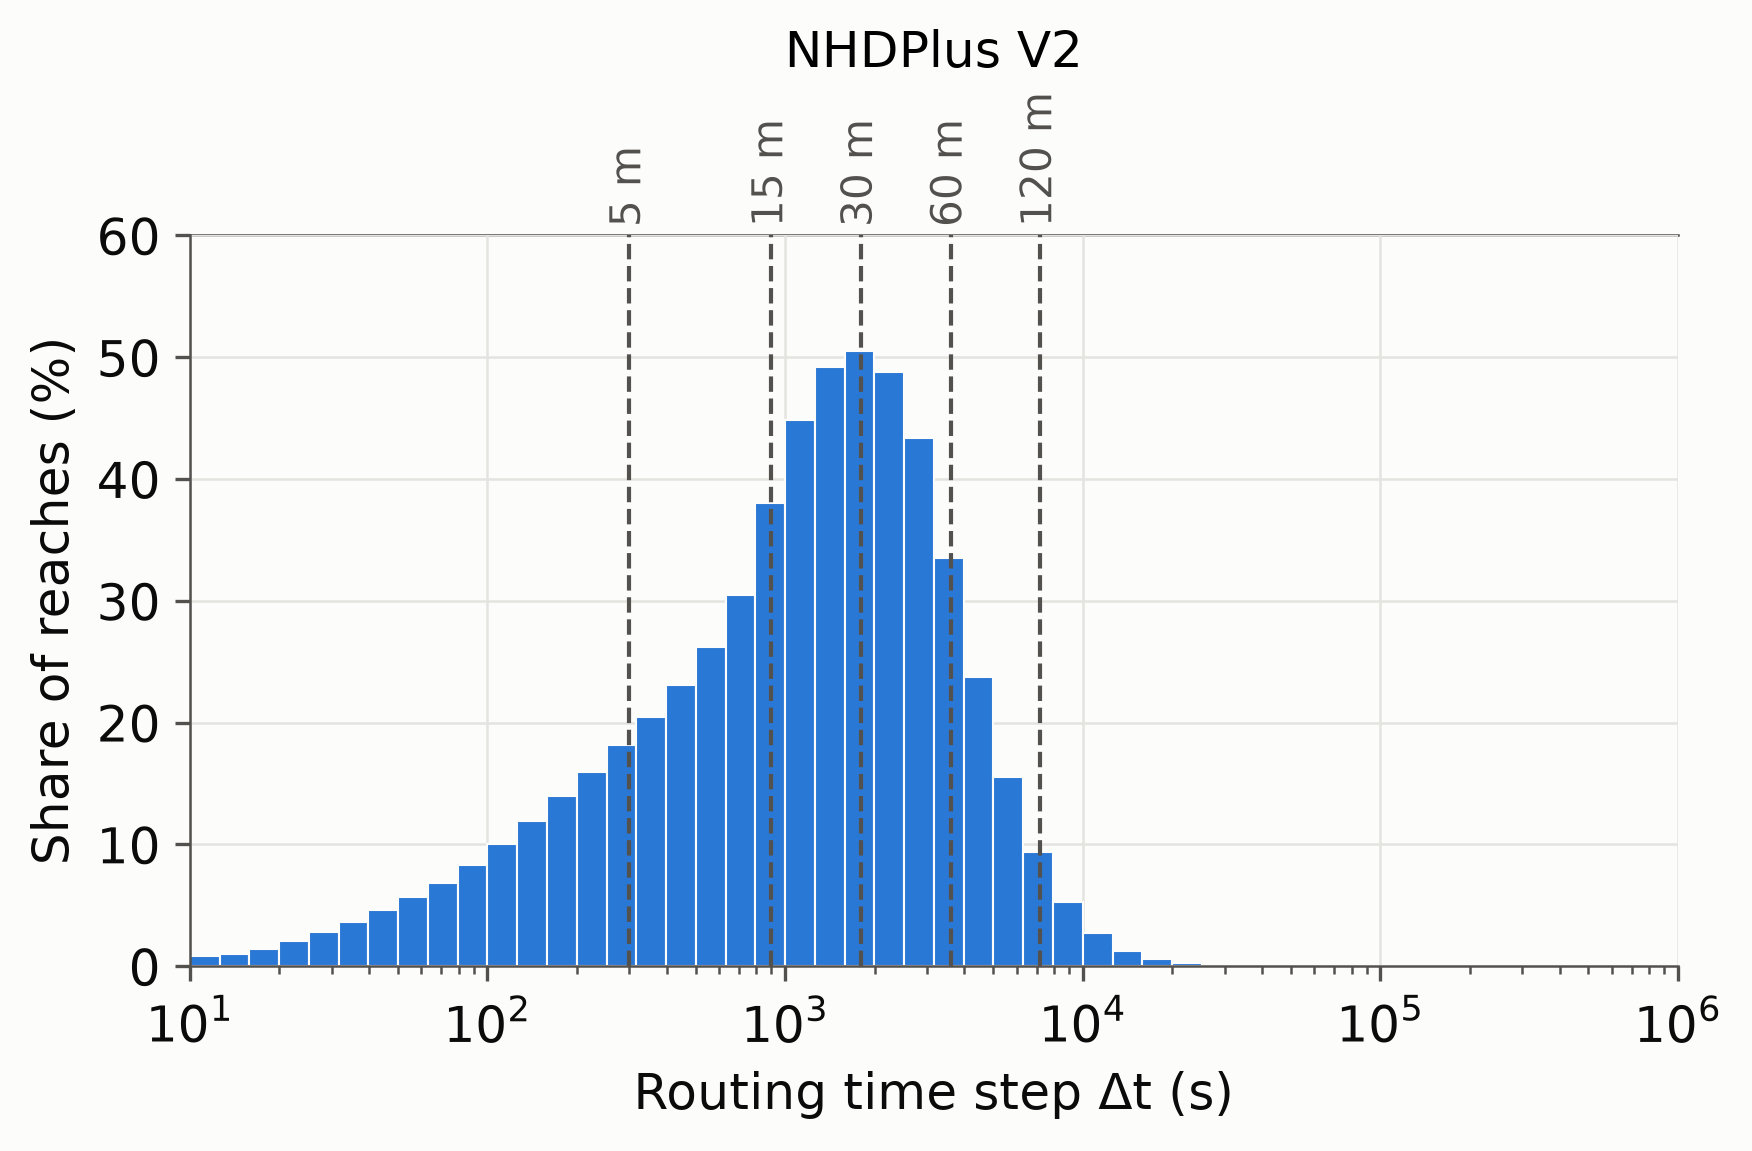
\includegraphics{../figures/dt_window_histogram_nhdplus-v2}
    \caption{Percentage of NHDPlus~V2 reaches with all positive Muskingum coefficients in each bin of routing time steps, assuming a constant flood wave celerity of 1~m/s and $x = 0.25$.}
    \label{fig:appendix-dt-window-nhdplus-v2}
\end{figure}

\begin{figure}[htbp]
    \centering
    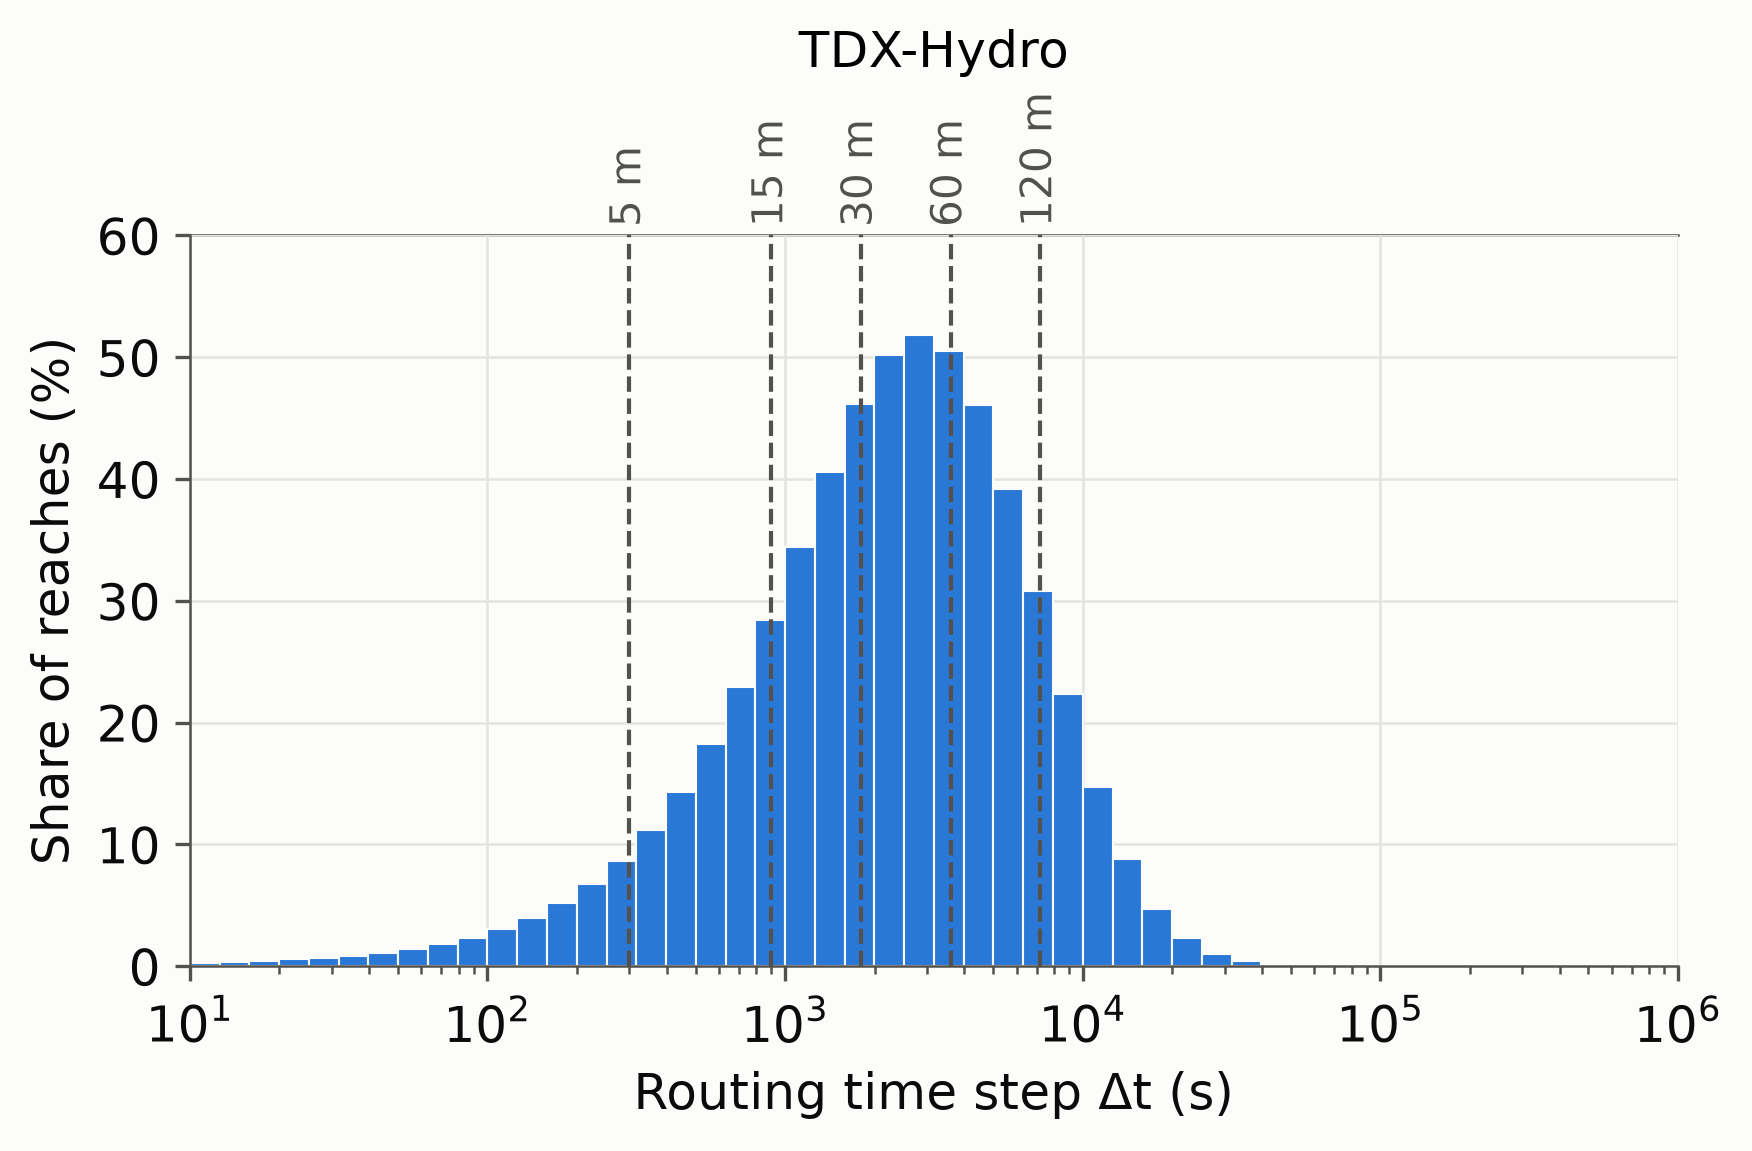
\includegraphics{../figures/dt_window_histogram_tdx-hydro}
    \caption{Percentage of TDX-Hydro reaches with all positive Muskingum coefficients in each bin of routing time steps, assuming a constant flood wave celerity of 1~m/s and $x = 0.25$.}
    \label{fig:appendix-dt-window-tdx-hydro}
\end{figure}

\begin{figure}[htbp]
    \centering
    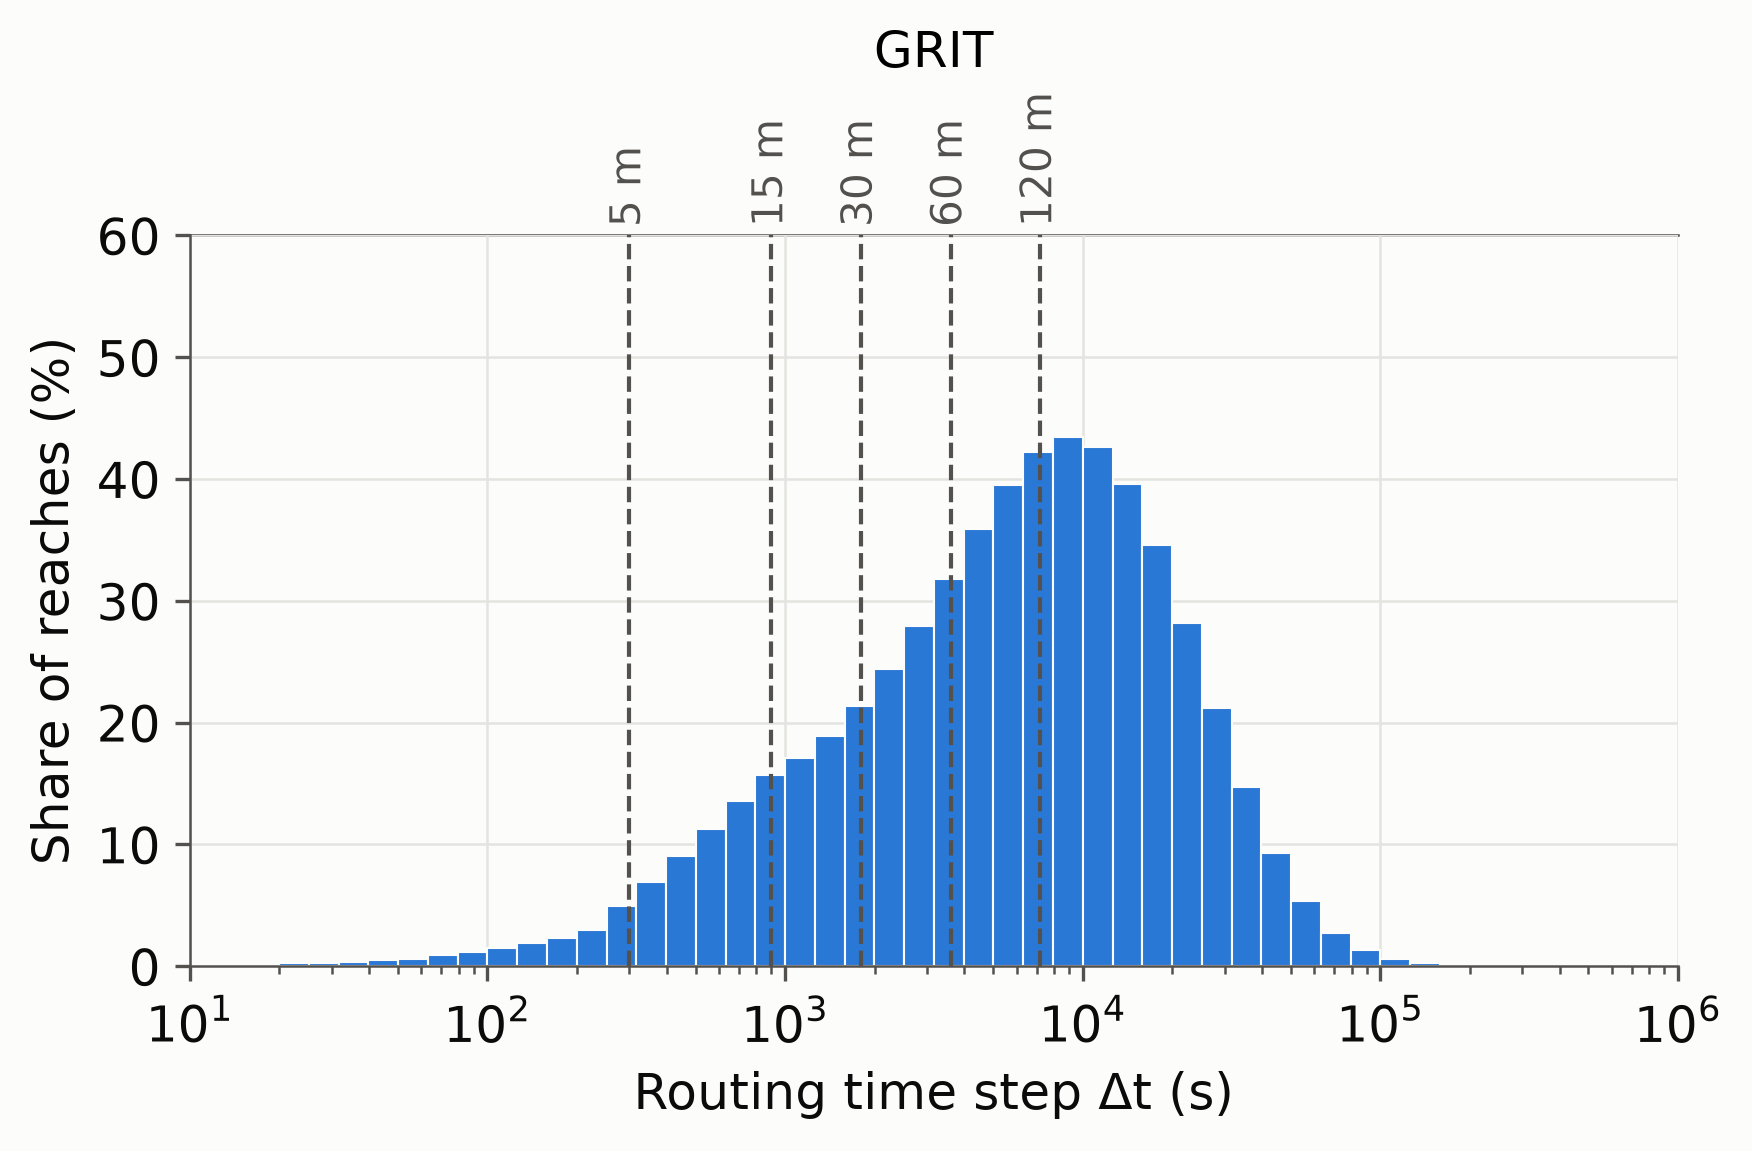
\includegraphics{../figures/dt_window_histogram_grit}
    \caption{Percentage of GRIT reaches with all positive Muskingum coefficients in each bin of routing time steps, assuming a constant flood wave celerity of 1~m/s and $x = 0.25$.}
    \label{fig:appendix-dt-window-grit}
\end{figure}

Figure~\ref{fig:appendix-dt-window-grid} tests the sensitivity of the combined histogram to the assumed celerity and to $x$.
Rows vary the celerity among 0.5, 1.0, and 1.5~m/s, and columns vary $x$ among 0.10, 0.25, and 0.40.
Changing the celerity scales every $k$ by the same factor, so it shifts the histogram along the logarithmic time step axis without changing its shape.
At $x = 0.25$, the time step valid for the most reaches moves from 53 to 66 minutes at 0.5~m/s to 21 to 26 minutes at 1.5~m/s, while the tallest bar stays at 46\% of reaches.
Changing $x$ changes the width of the range of valid time steps of each reach, which spans from $2kx$ to $2k(1-x)$, a factor of $(1-x)/x$.
That factor is 9 at $x = 0.10$, 3 at $x = 0.25$, and 1.5 at $x = 0.40$.
The tallest bar falls accordingly from 73\% to 46\% to 24\% of reaches at every celerity.
No combination of celerity and $x$ tested makes any time step valid for more than 73\% of reaches.

\begin{figure}[htbp]
    \centering
    \makebox[\textwidth][c]{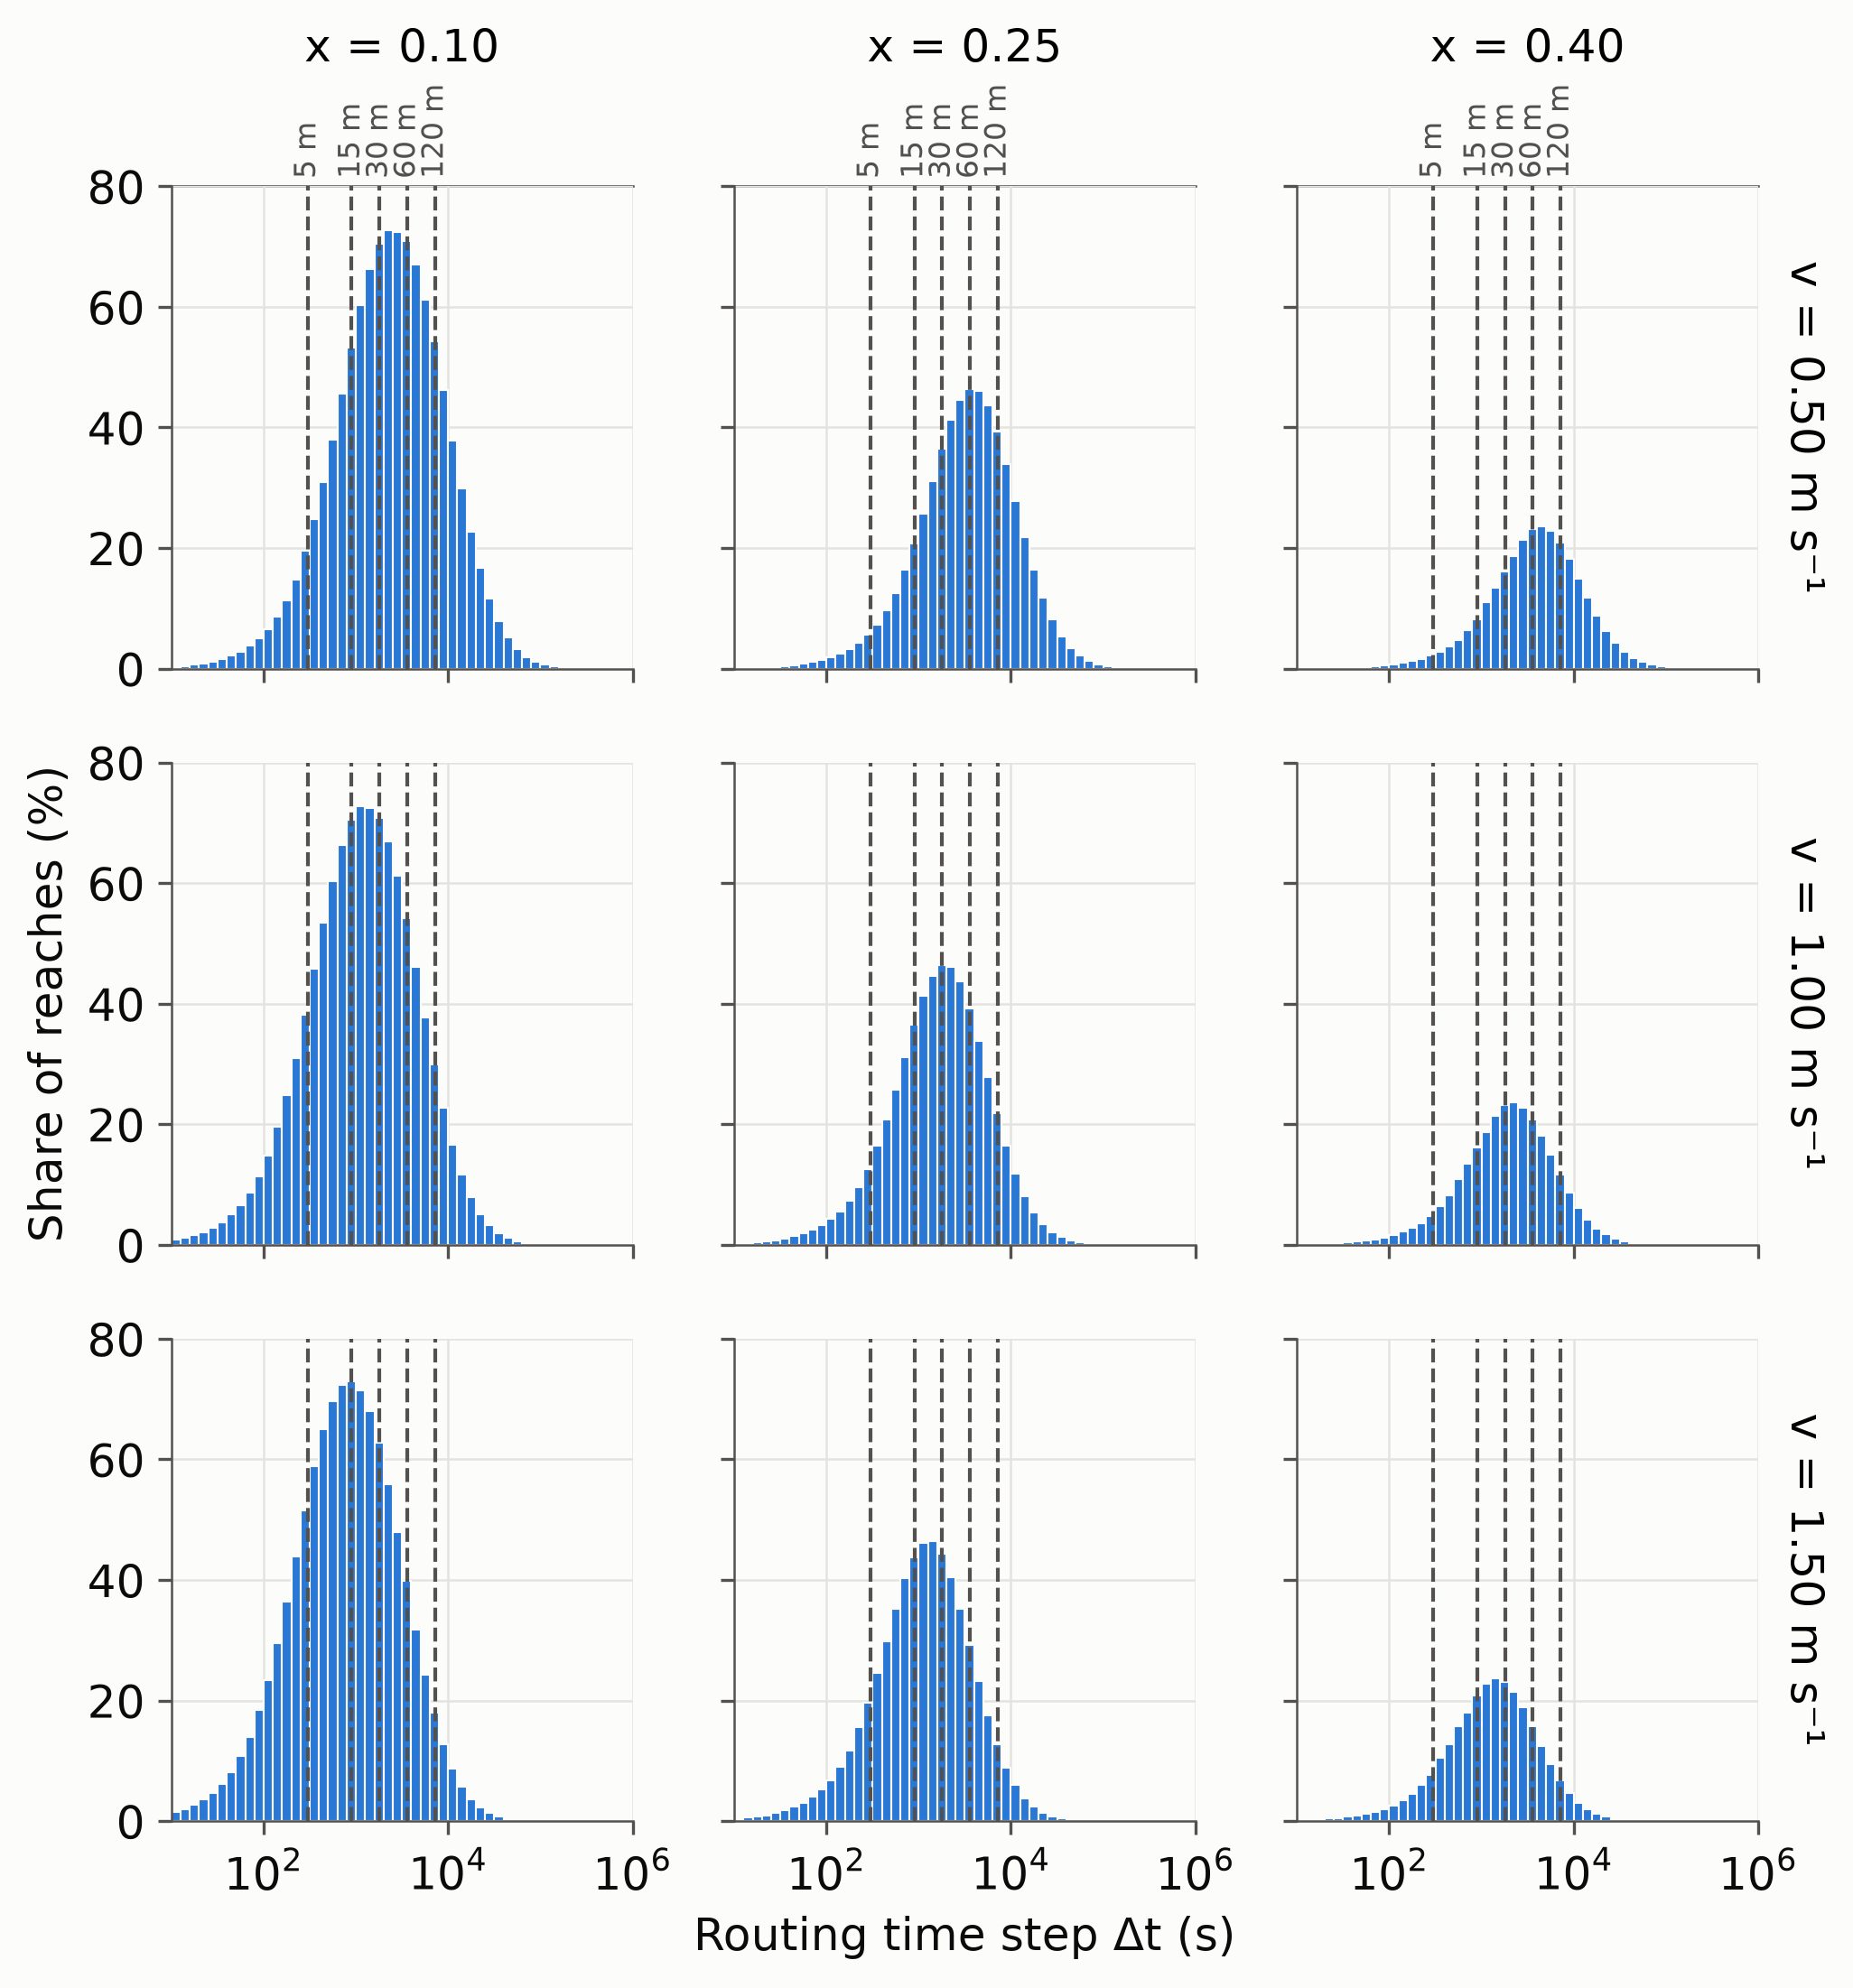
\includegraphics{../figures/dt_window_histogram_combined_grid}}
    \caption{Percentage of reaches of all six hydrography products combined with all positive Muskingum coefficients in each bin of routing time steps, at flood wave celerities of 0.5, 1.0, and 1.5~m/s (rows) and $x$ of 0.10, 0.25, and 0.40 (columns).}
    \label{fig:appendix-dt-window-grid}
\end{figure}

\clearpage
